\section{连续体的构型与运动描述}\label{content:coord}
在大变形下,连续体的未变形构型和变形构型存在巨大差异,因而需要对其做出明确区分。
通常如图~\ref{fig:config}~所示,取未发生变形的初始构型为参考构型,并用~$\BO$~表示;~
取变形后的构型为当前构型,并用~$\BT$~表示。

\begin{figure}[!h]
	\centering
	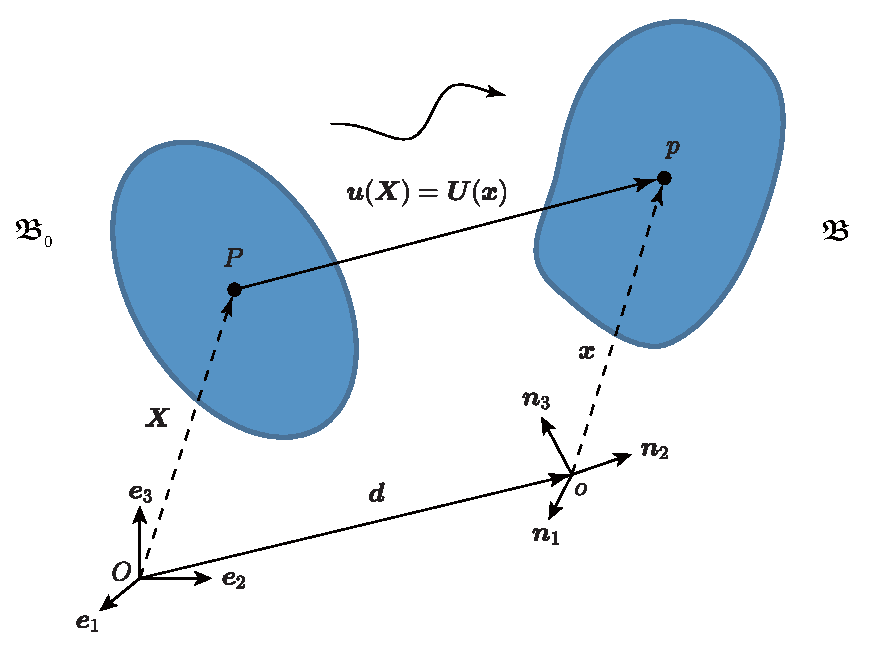
\includegraphics[scale=0.85]{configuaration.pdf}
	\caption{参考构型与当前构型}
	\label{fig:config}
\end{figure}

用于描述参考构型~$\BO$~的坐标系~$O-\bm{e}_1\bm{e}_2\bm{e}_3$~被称为物质坐标系,
用于描述当前构型~$\BT$~的坐标系~$o-\bm{n}_1\bm{n}_2\bm{n}_3$~被称为空间坐标系,
事实上这两种描述方法分别对应~Lagrange~描述法和~Euler~描述法。
下面考察图~\ref{fig:config}~中物质点~$P$~和空间点~$p$~(物质点~$P$~在空间中的位置)的运动学描述:
%--------------------------------
%--------------------------------
\begin{enumerate}
\item Lagrange~描述法\\
物质点~$P$~在当前构型~$\BT$~中的位置矢量~$\bm{x}$~是关于~$\bm{X}$~和~$t$~的函数
\begin{equation}\label{eq:config_L1}
	\bm{x}=\bm{x}(\bm{X},t)=x_i\bm{n}_i
\end{equation}
式中,$\bm{n}_i$~为空间坐标系的正交单位基矢量。\\
由式~\eqref{eq:config_L1}~可知,Lagrange~描述法是研究物质点的运动状态,
即同一物质点在不同时刻所对应的空间点。
同理,连接物质点~$P$~和空间点~$p$~的位移矢量,在~Lagrange~描述法下可表示为
\begin{equation}\label{eq:config_L2}
	\bm{u}=\bm{u}(\bm{X},t)=u_i\bm{n}_i
\end{equation}
同时位移矢量~$\bm{u}$~还可写作
\begin{equation}\label{eq:config_L3}
	\bm{u}(\bm{X},t)=\bm{d}(t)+\bm{x}(\bm{X},t)-\bm{X}
\end{equation}
式中,$\bm{d}(t)$~为刚体位移矢量。\\
将式~\eqref{eq:config_L3}~对位置矢量~$\bm{X}$~求偏导数,可得物质位移梯度张量
{\setlength\belowdisplayskip{5pt}
\begin{subequations}\label{eq:config_L4}
	\begin{align}
	\bm{u} \otimes \nabla_{\bm{X}} & =\bm{x} \otimes \nabla_{\bm{X}}-\bm{I} \label{eq:config_L4a} \\[1pt]
	\frac{\partial u_i}{\partial X_j} & =\frac{\partial x_i}{\partial X_j}-\delta_{ij} \label{eq:config_L4b}
	\end{align}
\end{subequations}}
式中,Hamiltonian~算符~$\nabla_{\bm{X}}=\DF{\partial}{\partial X_j} \bm{e}_j$~,
$\bm{I}$~为二阶单位张量。

需要注意到~$\bm{x} \otimes \nabla_{\bm{X}}=(\partial x_i \big/ \partial X_j)\bm{n}_i \otimes \bm{e}_j$~,
故在推导式~\eqref{eq:config_L4b}~中的分量形式时,假设了物质坐标系与空间坐标系的转移张量为~$\delta_{ij}=\bm{n}_i \cdot \bm{e}_j$~,
这表明物质坐标系与空间坐标系之间仅存在相对平移运动,而无任何相对刚体旋转运动,并在后续的论述中仍采用该假设。
%--------------------------------
%--------------------------------
\item Euler~描述法\\
空间点~$p$~在参考构型~$\BO$~中的位置矢量~$\bm{X}$~是关于~$\bm{x}$~和~$t$~的函数
\begin{equation}\label{eq:config_E1}
	\bm{X}=\bm{X}(\bm{x},t)=X_i\bm{e}_i
\end{equation}
式中,$\bm{e}_i$~是物质坐标系的正交单位基矢量。\\
由式~\eqref{eq:config_E1}~可知,Euler~描述法是研究空间点的运动状态,
即同一空间点在不同时刻所对应的物质点。
同理,连接物质点~$P$~和空间点~$p$~的位移矢量,在~Euler~描述法下可表示为
\begin{equation}\label{eq:config_E2}
	\bm{U}=\bm{U}(\bm{x},t)=U_i\bm{e}_i
\end{equation}
同时位移矢量~$\bm{U}$~还可写作
\begin{equation}\label{eq:config_E3}
	\bm{U}(\bm{x},t)=\bm{d}(t)+\bm{x}-\bm{X}(\bm{x},t)
\end{equation}
将式~\eqref{eq:config_E3}~对位置矢量~$\bm{x}$~求偏导数,可得空间位移梯度张量
{\setlength\belowdisplayskip{5pt}
\begin{subequations}\label{eq:config_E4}
	\begin{align}
	\bm{U} \otimes \nabla_{\bm{x}} & =\bm{I}-\bm{X} \otimes \nabla_{\bm{x}} \label{eq:config_E4a} \\[1pt]
	\frac{\partial U_i}{\partial x_j} & =\delta_{ij}-\frac{\partial X_i}{\partial x_j} \label{eq:config_E4b}
	\end{align}
\end{subequations}}
式中,Hamiltonian~算符~$\nabla_{\bm{x}}=\DF{\partial}{\partial x_j} \bm{n}_j$~,
且式~\eqref{eq:config_E4b}~中关于转移张量的定义与式~\eqref{eq:config_L4b}~一致。
\end{enumerate}

%----------------------------------------------------------------
\section{变形梯度}
\subsection{变形梯度的定义}
如图~\ref{fig:F}~所示,考虑参考构型~$\BO$~中的点~$P$~以及其邻域内的一点~$Q$~,
经历有限变形后得到当前构型~$\BT$~,同时点~$P$~、点~$Q$~移动到点~$p$~、点~$q$~,
于是可以得到有限变形前后的两个线元
\begin{subequations}\label{eq:line_x}
	\begin{align}
	\stackrel{\longrightarrow}{PQ} & =\diff \bm{X}=\diff X_i \bm{e}_i \label{eq:dX} \\
	\stackrel{\longrightarrow}{pq} & =\diff \bm{x}~=\diff x_i \bm{n}_i \label{eq:dx}
	\end{align}
\end{subequations}

\begin{figure}[!h]
	\centering
	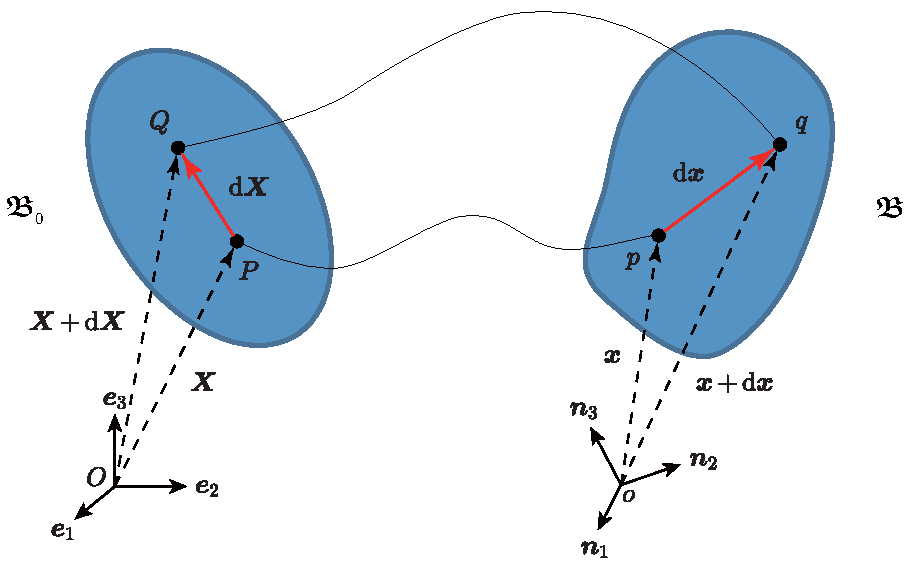
\includegraphics[scale=0.85]{deformation_gradient.pdf}
	\caption{连续体的变形}
	\label{fig:F}
\end{figure}

线元~$\diff \bm{X} \Rightarrow$~线元~$\diff \bm{x}$~经历了大小和方向的变化,
同样地,可以分别使用~Lagrange~描述法和~Euler~描述法来考察两者的变化规律:
%--------------------------------
%--------------------------------
\begin{enumerate}
\item Lagrange~描述法\\
在空间坐标系下,选取物质坐标~$\bm{X}$~作为自变量,
则物质点~$P$~、$Q$~在~$t$~时刻对应的空间点~$p$~、$q$~的坐标为
\begin{subequations}
	\begin{align}
	\bm{x} &=\bm{x} (\bm{X},t)  \\
	\bm{x}+\diff \bm{x}&=\bm{x} (\bm{X}+\diff \bm{X},t)
	\end{align}
\end{subequations}
将上两式作差可得
\begin{equation}\label{eq:trans_F}
	\diff \bm{x}=\bm{x} (\bm{X}+\diff \bm{X},t)-\bm{x} (\bm{X},t)=
	\frac{\partial \bm{x} (\bm{X})}{\partial \bm{X}} \cdot \diff \bm{X}
\end{equation}
式中,${\partial \bm{x} (\bm{X})}/{\partial \bm{X}}$~所定义的二阶张量被称为物质变形梯度张量,即
\begin{subequations}\label{eq:F}
	\begin{gather}
	\bm{F} = \bm{x} \otimes \nabla_{\bm{X}} = \frac{\partial \bm{x} (\bm{X})}{\partial \bm{X}} \\
	F_{ij} = \frac{\partial x_i}{\partial X_j}
	\end{gather}
\end{subequations}
将式~\eqref{eq:F}~所定义的变形梯度~$\bm{F}$~代入式~\eqref{eq:config_L4}~可得
\begin{equation}\label{eq:trans_u}
	\bm{F}=\bm{I}+\bm{u} \otimes \nabla_{\bm{X}}
\end{equation}
由上式可知,变形梯度~$\bm{F}$~包含了所有的有限变形信息,即大小和方向的变化。
%--------------------------------
%--------------------------------
\item Euler~描述法\\
在物质坐标系下,选取空间坐标~$\bm{x}$~作为自变量,则
空间点~$p$~、$q$~在~$t$~时刻对应的物质点~$P$~、$Q$~的坐标为
\begin{subequations}
	\begin{align}
	\bm{X} &=\bm{X} (\bm{x},t)  \\
	\bm{X}+\diff \bm{X}&=\bm{X} (\bm{x}+\diff \bm{x},t)
	\end{align}
\end{subequations}
将上两式作差可得
\begin{equation}
	\diff \bm{X}=\bm{X} (\bm{x}+\diff \bm{x},t)-\bm{X} (\bm{x},t)=
	\frac{\partial \bm{X} (\bm{x})}{\partial \bm{x}} \cdot \diff \bm{x}
\end{equation}
式中,${\partial \bm{X} (\bm{x})}/{\partial \bm{x}}$~所定义的二阶张量被称为空间变形梯度张量,即
\begin{subequations}\label{eq:F_inv}
	\begin{gather}
	\bm{F}^{-1} = \bm{X} \otimes \nabla_{\bm{x}} = \frac{\partial \bm{X} (\bm{x})}{\partial \bm{x}} \\
	F^{-1}_{ij} = \frac{\partial X_i}{\partial x_j}
	\end{gather}
\end{subequations}
将式~\eqref{eq:F_inv}~所定义的变形梯度~$\bm{F}^{-1}$~代入式~\eqref{eq:config_E4}~可得
\begin{equation}\label{eq:trans_u2}
	\bm{F}^{-1}=\bm{I}-\bm{U} \otimes \nabla_{\bm{x}}
\end{equation}
事实上,${\partial \bm{X} (\bm{x})}/{\partial \bm{x}}$~与~${\partial \bm{x} (\bm{X})}/{\partial \bm{X}}$~互逆,
故在式~\eqref{eq:F_inv}~中采用~$\bm{F}^{-1}$~的形式定义~${\partial \bm{X} (\bm{x})}/{\partial \bm{x}}$~,且未作特殊说明,一般将~$\bm{F}$~称为变形梯度。
\end{enumerate}

%----------------------------------------------------------------
\subsection{线元、面元、体元的变化}\label{content:dl}
下面具体考虑变形梯度~$\bm{F}$~对线元的长度和方向的影响,
设图~\ref{fig:F}~中线元~$\diff \bm{X}$~、$\diff \bm{x}$~表示为如下形式
\begin{subequations}\label{eq:dL}
	\begin{align}
	\diff \bm{X} & =\diff L ~\hat{\bm{N}} \\
	\diff \bm{x} & =\diff l ~\hat{\bm{n}} \label{eq:dL2}
	\end{align}
\end{subequations}
式中,$\diff L$~和~$\hat{\bm{N}}$~为参考构型~$\BO$~中线元的长度和单位方向矢量,
$\diff l$~和~$\hat{\bm{n}}$~为当前构型~$\BT$~中线元的长度和单位方向矢量。

将式~\eqref{eq:dL}~代入式~\eqref{eq:trans_F}~可得
\begin{subequations}
	\begin{align}
	\diff l ~\hat{\bm{n}} & = \bm{F} \cdot (\diff L ~\hat{\bm{N}}) \label{eq:dl1} \\
	\diff l ~\hat{\bm{n}} & = (\diff L ~\hat{\bm{N}}) \cdot \bm{F}^{\TT}
	\end{align}
\end{subequations}
将上两式作点积可得
\begin{subequations}\label{eq:trans_F2}
	\begin{equation}\label{eq:dldL}
	\lambda = \frac{\diff l}{\diff L} = \sqrt{ \hat{\bm{N}} \cdot (\bm{F}^{\TT} \cdot \bm{F}) \cdot \hat{\bm{N}} }
	\end{equation}
	将式~\eqref{eq:dldL}~代入式~\eqref{eq:dl1}~可得
	\begin{equation}
	\hat{\bm{n}} = \frac{1}{\sqrt{ \hat{\bm{N}} \cdot (\bm{F}^{\TT} \cdot \bm{F}) \cdot \hat{\bm{N}} }} (\bm{F} \cdot \hat{\bm{N}})
	\end{equation}
\end{subequations}
式中,$\lambda$~称为伸长比或长度比,上两式更具体地描述了有限变形前后线元的长度与方向的改变,
事实上式~\eqref{eq:trans_F}~与式~\eqref{eq:trans_F2}~是等价的关系。

\begin{figure}[!h]
	\centering
	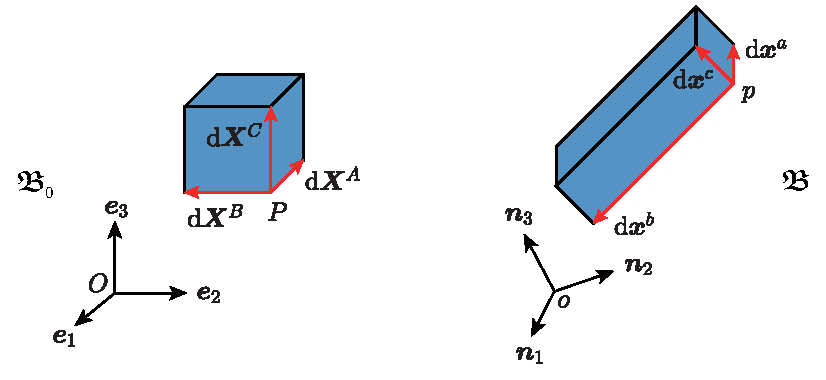
\includegraphics[scale=0.85]{det_F.pdf}
	\caption{变形前后的物质微元体}
	\label{fig:det_F}
\end{figure}

式~\eqref{eq:trans_F}~定义了线元~$\diff \bm{X}$~、$\diff \bm{x}$~之间的变换,同样地,可以考虑参考构型~$\BO$~和当前构型~$\BT$~中的体元、面元的变换关系。
如图~\ref{fig:det_F}~所示,在参考构型~$\BO$~中取微元体来研究变形梯度对体积的影响,
过物质点~$P$~取三个不共面的物质线元~$\diff \bm{X}^A$~、$\diff \bm{X}^B$~和~$\diff \bm{X}^C$~。
则在变形前,由这三个物质线元构成的平行六面体的体积为
\begin{equation}\label{eq:dVV}
	\begin{split}
	\diff V & =\diff \bm{X}^C \cdot (\diff \bm{X}^A \times \diff \bm{X}^B)\\
			& =(\diff X^C_k \bm{e}_k) \cdot \big[(\diff X^A_i \bm{e}_i) \times (\diff X^B_j \bm{e}_j)\big]\\
			& =\diff X^A_i \diff X^B_j \diff X^C_k \epsilon_{ijk}
	\end{split}
\end{equation}

经历有限变形后,线元~$\diff \bm{X}^A$~、$\diff \bm{X}^B$~、$\diff \bm{X}^C$~变为
~$\diff \bm{x}^a$~、$\diff \bm{x}^b$~、$\diff \bm{x}^c$~,则在当前构型~$\BT$~中微元体的体积为
\begin{equation}\label{eq:temp1}
	\diff v =\diff \bm{x}^c \cdot (\diff \bm{x}^a \times \diff \bm{x}^b)
\end{equation}
将式~\eqref{eq:trans_F}~代入式~\eqref{eq:temp1}~可得
\begin{equation}\label{eq:dv}
	\begin{split}
	\diff v & =(\bm{F} \cdot \diff \bm{X}^C) \cdot \big[(\bm{F} \cdot \diff \bm{X}^A) \times (\bm{F} \cdot \diff \bm{X}^B)\big]\\
			& =(F_{nk} \diff X^C_k \bm{e}_n) \cdot \big[(F_{li} \diff X^A_i \bm{e}_l) \times (F_{mj} \diff X^B_j \bm{e}_m)\big]\\
			& =F_{li} ~ F_{mj} F_{nk} \diff X^A_i \diff X^B_j \diff X^C_k \epsilon_{lmn}
	\end{split}
\end{equation}
考虑到行列式恒等式\cite{detF}
\begin{equation}\label{eq:detF}
	F_{li} ~ F_{mj} F_{nk} \epsilon_{lmn} = 
	\left|\begin{array}{ccc}
	F_{1i} & F_{2i} & F_{3i} \\
	F_{1j} & F_{2j} & F_{3j} \\
	F_{1k} & F_{2k} & F_{3k}
	\end{array}\right|
	=\det (\bm{F}) \epsilon_{ijk} = J \epsilon_{ijk}
\end{equation}
式中,$J$~为变形梯度~$\bm{F}$~的雅克比行列式。
将式~(\ref{eq:dVV})~、\eqref{eq:detF}~代入式~\eqref{eq:dv}~可得
\begin{equation}\label{eq:J}
	\diff v =J \diff X^A_i \diff X^B_j \diff X^C_k \epsilon_{ijk} = J \diff V
\end{equation}
式中,$J$~描述了有限变形前后微元体的体积比,且根据连续介质假设知~$J>0$~,即变形梯度~$\bm{F}$~是可逆的。

如图~\ref{fig:det_dA}~所示,考虑参考构型~$\BO$~和当前构型~$\BT$~中的两个面元,即
\begin{subequations}\label{eq:dA}
	\begin{align}
	\diff \bm{A} & =\diff A ~\bm{N} \\
	\diff \bm{a} & =\diff a ~\bm{n}
	\end{align}
\end{subequations}
式中,$\diff A$~和~$\bm{N}$~为参考构型~$\BO$~中面元的面积和单位外法线矢量,
$\diff a$和~$\bm{n}$~为当前构型~$\BT$~中面元的面积和单位外法线矢量。

\begin{figure}[!h]
	\centering
	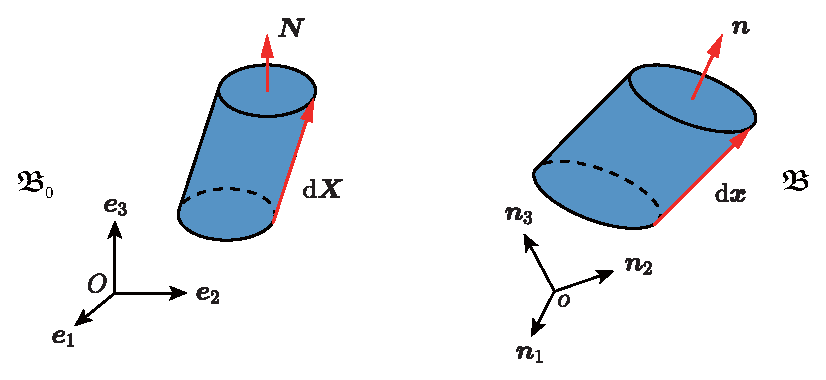
\includegraphics[scale=0.85]{det_dA.pdf}
	\caption{变形前后的面元}
	\label{fig:det_dA}
\end{figure}

在参考构型~$\BO$~中任取一个不正交于~$\bm{N}$~的线元~$\diff \bm{X}$~,即~$\bm{N} \cdot \diff \bm{X} \neq 0$~。
于是,将~$\diff A$~作为底面,$\diff \bm{X}$~作为母线,可作一个柱状微元体,其体积为
\begin{equation}\label{eq:dV1}
	\diff V = \diff \bm{A} \cdot \diff \bm{X} %= \diff A ~\bm{N} \cdot \diff \bm{X}
\end{equation}

参考构型~$\BO$~下的面元~$\diff \bm{A}$~经历有限变形后得到当前构型~$\BT$~下的面元~$\diff \bm{a}$~,
同时线元~$\diff \bm{X}$~变为~$\diff \bm{x}$~,于是可得变形后柱状微元体的体积
\begin{equation}\label{eq:dv1}
	\diff v = \diff \bm{a} \cdot \diff \bm{x}
\end{equation}
将式~\eqref{eq:dV1}~、\eqref{eq:dv1}~代入式~\eqref{eq:J}~可得
\begin{subequations}
	\begin{gather}
	\diff \bm{a} \cdot \diff \bm{x} = J \diff \bm{A} \cdot \diff \bm{X} \\
	\diff \bm{a} = J \diff \bm{A} \cdot \bm{F}^{-1} = J \bm{F}^{-\TT} \cdot \diff \bm{A} \label{eq:nanson}
	\end{gather}
\end{subequations}
式中,$\bm{F}^{-\TT}=(\bm{F}^{-1})^{\TT}=(\bm{F}^{\TT})^{-1}$~。
式~\eqref{eq:nanson}~被称为~Nanson~公式,该公式给定了面元的面积和方向在有限变形前后的关系。

将式~\eqref{eq:dA}~代入式~\eqref{eq:nanson}~可得
\begin{subequations}
	\begin{align}
	\diff a ~\bm{n} & = J (\diff A ~\bm{N}) \cdot \bm{F}^{-1} = J \diff A (\bm{N} \cdot \bm{F}^{-1}) \label{eq:dandAN} \\
	\diff a ~\bm{n} & = J \bm{F}^{-\TT} \cdot (\diff A ~\bm{N}) = J \diff A (\bm{F}^{-\TT} \cdot \bm{N})
	\end{align}
\end{subequations}
将上两式作点积可得
\begin{subequations}\label{eq:nanson2}
	\begin{equation}\label{eq:dadA}
	\frac{\diff a}{\diff A} = J \sqrt{ \bm{N} \cdot (\bm{F}^{\TT} \cdot \bm{F})^{-1} \cdot \bm{N} }
	\end{equation}
	将式~\eqref{eq:dadA}~代入式~\eqref{eq:dandAN}~可得
	\begin{equation}
	\bm{n} = \frac{1}{\sqrt{ \bm{N} \cdot (\bm{F}^{\TT} \cdot \bm{F})^{-1} \cdot \bm{N} }} (\bm{N} \cdot \bm{F}^{-1})
	\end{equation}
\end{subequations}
上两式更具体地描述了有限变形前后面元的面积与方向的改变,
事实上式~\eqref{eq:nanson}~与式~\eqref{eq:nanson2}~是等价的关系。

综上,式~\eqref{eq:trans_F}~和式~\eqref{eq:trans_F2}~、式~\eqref{eq:nanson}~和式~\eqref{eq:nanson2}~、
式~\eqref{eq:J}~分别对应有限变形前后线元、面元、体元的关系,从一个侧面说明了变形梯度~$\bm{F}$~可以描述有限变形的全部信息。

%----------------------------------------------------------------
\subsection{变形梯度的极分解}
任意二阶可逆张量都可以分解为一个对称正定张量与一个正交张量的乘积,数学上将其称为极分解定理\cite{polar}。
如图~\ref{fig:polar_decomp}~所示,在连续介质力学的框架下,变形梯度~$\bm{F}$~也可被分解为代表刚体旋转的正交张量与代表纯粹变形的对称正定张量,
其数学形式如下
\begin{equation}\label{eq:polar_decomp}
	\bm{F}=\bm{R} \cdot \bm{U} = \bm{V} \cdot \bm{R}
\end{equation}
式中,$\bm{R}$~为正交张量,$\bm{U}$~和~$\bm{V}$~为对称正定张量,
通常将张量~$\bm{U}$~、$\bm{V}$~分别称为右、左拉伸张量,且上式中的极分解是唯一的。
由式~\eqref{eq:polar_decomp}~不难得出
\begin{subequations}\label{eq:UUVV}
	\begin{align}
	\bm{U}^2 & =\bm{F}^{\TT} \cdot \bm{F} \\
	\bm{V}^2 & =\bm{F} \cdot \bm{F}^{\TT}
	\end{align}
\end{subequations}

\begin{figure}[!h]
	\centering
	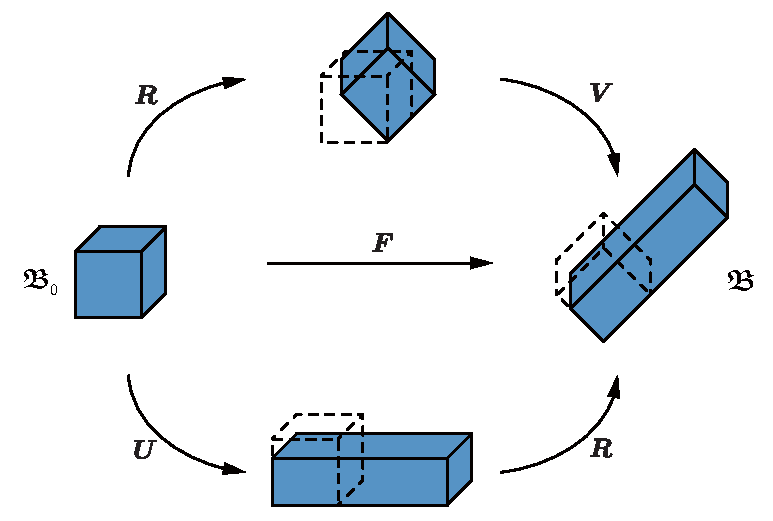
\includegraphics[scale=0.85]{polar_decomposition.pdf}
	\caption{变形梯度~$\bm{F}$~的极分解}
	\label{fig:polar_decomp}
\end{figure}

单纯的旋转不会在变形体中引起任何应变,因而在连续介质力学中需要使用与旋转无关的量来衡量变形。
在式~\eqref{eq:UUVV}~中利用变形梯度~$\bm{F}$~与其转置相乘来消除旋转张量~$\bm{R}$~的影响,
于是可以引入两种的变形张量 
\begin{subequations}
	\begin{align}
	\bm{C} & =\bm{F}^{\TT} \cdot \bm{F} \label{eq:CeqFTF} \\
	\bm{B} & =\bm{F} \cdot \bm{F}^{\TT} \label{eq:BeqFFT}
	\end{align}
\end{subequations}
式中,张量~$\bm{C}$~被称为右~Cauchy~-~Green~变形张量或~Green~变形张量,
张量~$\bm{B}$~被称为左~Cauchy~-~Green~变形张量,$\bm{B}^{-1}$~被称为~Cauchy~变形张量,
且~$\bm{C}$~、$\bm{B}$~均为对称正定张量。

%----------------------------------------------------------------
\section{应力应变描述}
\subsection{应变张量的描述}\label{content:strain}
在~\ref{content:dl}~条中研究了线元的变化,考虑到式~\eqref{eq:CeqFTF}~的定义,
可将式~\eqref{eq:dldL}~改写为
\begin{subequations}
	\begin{gather}
	(\diff L)^2 = \diff \bm{X} \cdot \diff \bm{X} = \diff X_i \diff X_i  \\
	(\diff l)^2 = \diff \bm{x} \cdot \diff \bm{x} =\diff \bm{X} \cdot \bm{C} \cdot \diff \bm{X} = C_{ij} \diff X_i \diff X_j \label{eq:dl^2}
	\end{gather}
\end{subequations}
将上两式作差可得
\begin{equation}
	(\diff l)^2-(\diff L)^2=\diff \bm{X} \cdot (\bm{C}-\bm{I}) \cdot \diff \bm{X}=(C_{ij}-\delta_{ij}) \diff X_i \diff X_j
\end{equation}
当连续体没有发生变形时,即~$\diff L =\diff l$~,则由上式易知~$\bm{C}-\bm{I}=\bm{0}$~,
故可以选取~$\bm{C}-\bm{I}$~来衡量有限应变。通常可引入~Green~应变张量
\begin{equation}\label{eq:strain_E}
	\bm{E}=\frac{1}{2}(\bm{C}-\bm{I})=\frac{1}{2}(\bm{F}^{\TT} \cdot \bm{F}-\bm{I})
\end{equation}
将式~\eqref{eq:trans_u}~代入式~\eqref{eq:strain_E}~,以物质位移梯度张量来表征应变张量
{\setlength\belowdisplayskip{5pt}
\begin{subequations}\label{eq:strain_E2}
	\begin{align}
	\bm{E}  & =\frac{1}{2}(\bm{F}^{\TT} \cdot \bm{F}-\bm{I}) \notag \\[5pt]
			& =\frac{1}{2}\left[(\bm{I}+\nabla_{\bm{X}} \otimes \bm{u}) \cdot (\bm{I}+\bm{u} \otimes \nabla_{\bm{X}}) - \bm{I}\right] \\[5pt]
			& =\frac{1}{2}\left[\bm{u} \otimes \nabla_{\bm{X}} + \nabla_{\bm{X}} \otimes \bm{u} + (\nabla_{\bm{X}} \otimes \bm{u}) \cdot (\bm{u} \otimes \nabla_{\bm{X}}) \right] \notag \\[5pt]
	E_{ij}  & =\frac{1}{2} \left( \frac{\partial u_i}{\partial X_j} + \frac{\partial u_j}{\partial X_i} + \frac{\partial u_k}{\partial X_i} \frac{\partial u_k}{\partial X_j}\right) \label{eq:strain_E3}
	\end{align}
\end{subequations}}
式中,应变张量~$\bm{E}$~是在物质坐标系下描述的,故也被称为~Lagrange~应变张量。

类似地,可以引入~Almansi~应变张量
\begin{equation}\label{eq:strain_e}
	\bm{e}=\frac{1}{2}(\bm{I}-\bm{B}^{-1})=\frac{1}{2}(\bm{I}-\bm{F}^{-\TT} \cdot \bm{F}^{-1})
\end{equation}
将式~\eqref{eq:trans_u2}~代入式~\eqref{eq:strain_e}~,以空间位移梯度张量来表征应变张量
{\setlength\belowdisplayskip{5pt}
\begin{subequations}\label{eq:strain_e2}
	\begin{align}
	\bm{e}  & =\frac{1}{2}(\bm{I}-\bm{F}^{-\TT} \cdot \bm{F}^{-1}) \notag \\[5pt]
			& =\frac{1}{2}\left[\bm{I} - (\bm{I}-\nabla_{\bm{x}} \otimes \bm{U}) \cdot (\bm{I}-\bm{U} \otimes \nabla_{\bm{x}}) \right] \\[5pt]
			& =\frac{1}{2}\left[\bm{U} \otimes \nabla_{\bm{x}} + \nabla_{\bm{x}} \otimes \bm{U} - (\nabla_{\bm{x}} \otimes \bm{U}) \cdot (\bm{U} \otimes \nabla_{\bm{x}}) \right] \notag \\[5pt]
	e_{ij}  & =\frac{1}{2} \left( \frac{\partial U_i}{\partial x_j} + \frac{\partial U_j}{\partial x_i} - \frac{\partial U_k}{\partial x_i} \frac{\partial U_k}{\partial x_j}\right) \label{eq:strain_e3}
	\end{align}
\end{subequations}}
式中,应变张量~$\bm{e}$~是在空间坐标系下描述的,故也被称为~Euler~应变张量。

由式~\eqref{eq:strain_E}~、\eqref{eq:strain_e}~不难得出
\begin{equation}\label{eq:trans_E_e}
	\bm{E}=\bm{F}^{\TT} \cdot \bm{e} \cdot \bm{F}
\end{equation}
上式表明,应变张量~$\bm{E}$~和~$\bm{e}$~满足特定的变换关系。
具体而言,应变张量在空间坐标系中的分量所对应的矩阵为~$\bm{e}$~,
而在物质坐标系中的分量所对应的矩阵恰好等于~$\bm{E}$~。

对于一般的微小变形,可以略去式~\eqref{eq:strain_E2}~、\eqref{eq:strain_e2}~中的二阶小量,
同时忽略不同构型之间的坐标系差异,可以得到经典的小应变公式
{\setlength\belowdisplayskip{5pt}
\begin{subequations}
	\begin{align}
	\bm{\varepsilon} & = \frac{1}{2}\left(\bm{u} \otimes \nabla_{\bm{x}} + \nabla_{\bm{x}} \otimes \bm{u} \right) \\[5pt]
	\varepsilon_{ij} & = \frac{1}{2}\left(\frac{\partial u_i}{\partial x_j} + \frac{\partial u_j}{\partial x_i} \right)
	\end{align}
\end{subequations}}
显然,在有限变形下不能忽略二阶项带来的影响,有限应变张量正是对小应变公式的一种修正。

除了上述的两种应变张量外,还有名义应变张量和对数应变张量等。
其中,名义应变张量又称~Biot~应变张量,其数学形式如下
\begin{equation}
	\bm{E}^{B}=\bm{U}-\bm{I}
\end{equation}
对数应变张量又分~Logarithmic~应变张量与~Hencky~应变张量,其数学形式如下
\begin{subequations}
	\begin{align}
	\bm{E}^{L} & =\mathrm{ln} ~ \bm{U} \\
	\bm{e}^{H} & =\mathrm{ln} ~ \bm{V}
	\end{align}
\end{subequations}

%----------------------------------------------------------------
\subsection{应力张量的描述}
文献\cite{jinming}中引入了~Cauchy~应力张量的概念,并指出该张量为二阶张量,且作用在当前构型~$\BT$~上,
通常将其记为
\begin{equation}
	\bm{\sigma}=\sigma_{ij} \bm{n}_i \otimes \bm{n}_j
\end{equation}
式中,$\sigma_{11}$~、$\sigma_{22}$~、$\sigma_{33}$~对应正应力,
~$\sigma_{12}$~、$\sigma_{13}$~、$\sigma_{23}$~对应剪应力,
且~$\bm{\sigma}^{\TT}=\bm{\sigma}$~。

如图~\ref{fig:cauchy_stress}~所示,任意四面体微元的应力状态由~Cauchy~应力张量~$\bm{\sigma}$~表征,
四面体微元的斜平面单位外法线矢量为~$\bm{n}$~,该斜平面上的应力矢量为~$\bm{t}$~。
上述三个量存在一个简单的数学关系,冯元桢\cite{fyz}给出了一种初等证明方法,其最终形式如下
\begin{subequations}\label{eq:cauchy_stress}
	\begin{align}
	\bm{t} & =\bm{\sigma} \cdot \bm{n} \label{eq:cauchy_stress1} \\
	   t_i & =\sigma_{ij} n_j
	\end{align}
\end{subequations}
上式又被称为~Cauchy~公式。

\begin{figure}[!h]
	\centering
	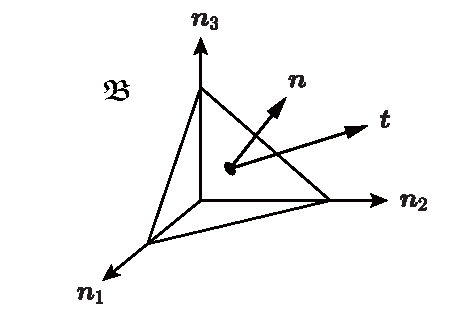
\includegraphics[scale=0.85]{cauchy_stress.pdf}
	\caption{四面体表面上的应力矢量~$\bm{t}$~}
	\label{fig:cauchy_stress}
\end{figure}

除了~Cauchy~应力张量之外,在当前构型~$\BT$~中还可定义~Kirchhoff~应力张量
\begin{equation}\label{eq:kirchhoff_stress}
	\bm{\tau}=J \bm{\sigma}
\end{equation}
式中,$J=\det (\bm{F})$~,且该应力张量常用于数值计算。

~Cauchy~应力张量~$\bm{\sigma}$~和~Kirchhoff~应力张量~$\bm{\tau}$~都是作用在当前构型~$\BT$~上的,
事实上如图~\ref{fig:det_dA}~所示,在有限变形中当前构型~$\BT$~的边界是未知的,
所以式~\eqref{eq:cauchy_stress1}~中的~$\bm{n}$~也是未知的。
相反地,在参考构型~$\BO$~中,面元~$\diff \bm{A}$~的单位外法线矢量~$\bm{N}$~是容易根据已知的几何边界来确定的。
考虑到在变形前后面元上的力系主矢是相等的,则由式~\eqref{eq:cauchy_stress}~可得
\begin{equation}\label{eq:piola1}
	(\bm{P} \cdot \bm{N})\diff A=(\bm{\sigma} \cdot \bm{n})\diff a
\end{equation}
式中,$\bm{P}$~为作用在参考构型~$\BO$~上的应力张量。
将式~\eqref{eq:dA}~、\eqref{eq:nanson}~代入式~\eqref{eq:piola1}~可得
\begin{equation}\label{eq:piola2}
	\bm{P} \cdot \diff \bm{A}=J \bm{\sigma} \cdot \bm{F}^{-\TT} \cdot \diff \bm{A}
\end{equation}
考虑到面元~$\diff \bm{A}$~的任意性,故必有
\begin{equation}\label{eq:piola3}
	\bm{P}=J \bm{\sigma} \cdot \bm{F}^{-\TT}
\end{equation}
式中,二阶张量~$\bm{P}$~被称为第一类~Piola~-~Kirchhoff~应力张量。

由式~\eqref{eq:piola3}~易知,虽然~Cauchy~应力张量~$\bm{\sigma}$~是对称的,
但是第一类~Piola~-~Kirchhoff~应力张量~$\bm{P}$~却不一定是对称的。
故而将式~\eqref{eq:piola3}~左点积~$\bm{F}^{-1}$~,得到
\begin{equation}\label{eq:piola4}
	\bm{S}=\bm{F}^{-1} \cdot \bm{P}=J \bm{F}^{-1} \cdot \bm{\sigma} \cdot \bm{F}^{-\TT}
\end{equation}
式中,对称二阶张量~$\bm{S}$~被称为第二类~Piola~-~Kirchhoff~应力张量。

%----------------------------------------------------------------
\section{变形的率形式描述}
\subsection{速度梯度}
在研究连续体的变形运动过程时,需要知道位置~$\bm{x}(t)$~、速度~$\bm{v}(t)$~等信息来描述其运动状态。
在空间坐标系下,考虑物质坐标为~$\bm{X}$~和~$\bm{X}+\diff \bm{X}$~的两点,则其在~$t$~时刻对应的速度为
\begin{subequations}
	\begin{gather}
	\bm{v} = \bm{v} (\bm{x}(\bm{X}),t) = \frac{\partial \bm{x} (\bm{X},t)}{\partial t} \\[5pt]
	\bm{v}+\diff \bm{v} = \bm{v} (\bm{x}(\bm{X}+\diff \bm{X}),t) = \frac{\partial \bm{x} (\bm{X}+\diff \bm{X},t)}{\partial t}
	\end{gather}
\end{subequations}
将上两式作差可得
\begin{equation}\label{eq:grad_v}
	\diff \bm{v}=\bm{v} (\bm{x}(\bm{X}+\diff \bm{X}),t) - \bm{v} (\bm{x}(\bm{X}),t)=
	\frac{\partial \bm{v}(\bm{x})}{\partial \bm{x}} \cdot \diff \bm{x}
\end{equation}
式中,${\partial \bm{v} (\bm{x})}/{\partial \bm{x}}$~所定义的二阶张量被称为速度梯度张量,即
\begin{subequations}\label{eq:L}
	\begin{gather}
	\bm{L} = \bm{v} \otimes \nabla_{\bm{x}} = \frac{\partial \bm{v} (\bm{x})}{\partial \bm{x}} \\
	L_{ij} = \frac{\partial v_i}{\partial x_j}
	\end{gather}
\end{subequations}

初始构型~$\BO$~中的线元~$\diff \bm{X}$~在经过时间~$t$~后变为当前构型~$\BT$~中的线元~$\diff \bm{x}$~,
考虑到式~\eqref{eq:trans_F}~,并对线元~$\diff \bm{x}$~求物质导数,则有
\begin{subequations}\label{eq:grad_v2}
\begin{equation}\label{eq:grad_v3}
	\frac{\partial}{\partial t}(\diff \bm{x}) = \frac{\partial \bm{F}}{\partial t} \cdot \diff \bm{X} ~~\Rightarrow~~
	\diff \bm{v} = \dot{\bm{F}} \cdot \bm{F}^{-1} \cdot \diff \bm{x}
\end{equation}
式中,
\begin{equation}\label{eq:grad_v4}
	\dot{\bm{F}} \cdot \bm{F}^{-1} = \frac{\partial}{\partial t} \left( \frac{\partial \bm{x}}{\partial \bm{X}} \right)
	\cdot \frac{\partial \bm{X}}{\partial \bm{x}} = \frac{\partial}{\partial \bm{X}} \left( \frac{\partial \bm{x}}{\partial t} \right)
	\cdot \frac{\partial \bm{X}}{\partial \bm{x}} = \frac{\partial \bm{v}}{\partial \bm{X}} \cdot \frac{\partial \bm{X}}{\partial \bm{x}} = 
	\frac{\partial \bm{v}}{\partial \bm{x}}
\end{equation}
\end{subequations}
于是,由式~\eqref{eq:grad_v}~、\eqref{eq:grad_v2}~可知
\begin{equation}\label{eq:L2}
	\bm{L} = \dot{\bm{F}} \cdot \bm{F}^{-1}
\end{equation}
上式表明,速度梯度张量~$\bm{L}$~可以根据变形梯度张量~$\bm{F}$~表示出来。

下面研究变形梯度张量~$\bm{F}$~的雅可比行列式~$J$~对时间~$t$~的导数~,
首先根据文献\cite{shulijichu}中的结论,即
\begin{equation}\label{eq:adjA}
	\frac{\partial |\bm{F}|}{\partial F_{ij}} = (\bm{F}^*)_{ji} = |\bm{F}| ~ (\bm{F}^{-1})_{ji}
\end{equation}
式中,$\bm{F}^* = \mathrm{adj}(\bm{F})$~,即~$\bm{F}$~的伴随矩阵,下标~$ji$~表示其~$j$~行、$i$~列的分量,
于是~$(\bm{F}^*)_{ji}$~为元素~$F_{ij}$~所对应的代数余子式,则该式表明代数余子式可以表示为行列式的偏导数。

由式~\eqref{eq:adjA}~可作如下推导
\begin{equation} \label{eq:dJdt}
\begin{split}
	\frac{\diff |\bm{F}|}{\diff t} & = \frac{\partial |\bm{F}|}{\partial F_{ij}} \frac{\partial F_{ij}}{\partial t} 
									 = |\bm{F}| ~ (\bm{F}^{-1})_{ji} \frac{\partial F_{ij}}{\partial t}  \\
								   & = |\bm{F}| ~ \trd(\bm{F}^{-1} \cdot \dot{\bm{F}}) 
								     = |\bm{F}| ~ \trd(\dot{\bm{F}} \cdot \bm{F}^{-1})  \\
							       & = |\bm{F}| ~ \trd(\bm{L})
\end{split}
\end{equation}
考虑到式~\eqref{eq:D}~的定义,可将式~\eqref{eq:dJdt}~进一步写作
\begin{subequations} \label{eq:dJdt2}
\begin{gather}
	\dot{J} = J~ \trd(\bm{L}) = J~ \trd(\bm{D}) = J~ \nabla_{\bm{x}} \cdot \bm{v} \\
	\dot{J} = J~L_{ii} = J~D_{ii} = J~{\partial v_i}/{\partial x_i}
\end{gather}
\end{subequations}
式~\eqref{eq:dJdt2}~表明,微元体单位体积的体积对时间变化率等于速度矢量的散度,
事实上该式揭示了连续体在变形过程中需要满足质量守恒定律,即
\begin{equation}\label{eq:dJdt3}
	\frac{\diff}{\diff t}(\rho J) = \dot{\rho} ~J+\rho ~\dot{J} = 0 ~~\Rightarrow~~
	\dot{\rho}+\rho ~ \nabla_{\bm{x}} \cdot \bm{v} = 0
\end{equation}
式中,$\rho$~为连续体密度,上式也被称为连续性方程。

%----------------------------------------------------------------
\subsection{变形率与自旋率张量}
考察~$t$~时刻当前构型~$\BT$~中的线元~$\diff \bm{x}$~,并按照式~\eqref{eq:dL2}~定义其长度与方向,
在~$t+\diff t$~时刻线元~$\diff \bm{x}$~的长度变为
\begin{equation}\label{eq:dL3}
	\diff \tilde{l} =\diff l +\diff ( \diff l )
\end{equation}
则在~$\diff t$~的时间内可以定义线元~$\diff \bm{x}$~的线应变率,即
\begin{equation}\label{eq:line_e}
	\dot{\varepsilon}=\frac{\diff \tilde{l}-\diff l}{\diff l} \frac{1}{\diff t}=\frac{1}{\diff l} \frac{\diff (\diff l)}{\diff t} =
	\frac{1}{\diff l} \frac{\partial (\diff l)}{\partial t}
\end{equation}
式中,$\dot{\varepsilon}$~也被称为伸长率,用来衡量线元~$\diff \bm{x}$~长度的变化速率,且为一标量。

为了得出线应变率~$\dot{\varepsilon}$~,将式~\eqref{eq:dl^2}~对时间~$t$~求偏导数,即
\begin{subequations}\label{eq:line_e2}
\begin{equation}\label{eq:line_e3}
	\frac{\partial (\diff l)^2}{\partial t} = \frac{\partial}{\partial t}(\diff \bm{x} \cdot \diff \bm{x}) ~~\Rightarrow~~
	2 \diff l ~\frac{\partial}{\partial t}(\diff l) =
	\frac{\partial}{\partial t}(\diff \bm{x}) \cdot \diff \bm{x} + \diff \bm{x} \cdot \frac{\partial}{\partial t}(\diff \bm{x})
\end{equation}
式中,
\begin{equation}\label{eq:line_e4}
	\frac{\partial}{\partial t}(\diff \bm{x}) = \diff \dot{\bm{x}} =
	\frac{\partial \bm{v}}{\partial \bm{x}} \cdot \diff \bm{x} =
	\bm{L} \cdot \diff \bm{x}
\end{equation}
将式~\eqref{eq:line_e4}~代入式~\eqref{eq:line_e3}~可得
\begin{equation}\label{eq:line_e5}
	2 \diff l ~\frac{\partial}{\partial t}(\diff l) =\diff \bm{x} \cdot (\bm{L}+\bm{L}^{\TT}) \cdot \diff \bm{x}
\end{equation}
于是,由式~\eqref{eq:dL2}~、\eqref{eq:line_e}~和~\eqref{eq:line_e5}~可得
\begin{equation}\label{eq:line_e6}
	\dot{\varepsilon}=\hat{\bm{n}} \cdot \frac{\bm{L}+\bm{L}^{\TT}}{2} \cdot \hat{\bm{n}}
\end{equation}
\end{subequations}
通常将速度梯度张量~$\bm{L}$~的对称部分定义为变形率张量,即
\begin{subequations}\label{eq:D}
	\begin{gather}
	\bm{D} = \mathrm{symm}(\bm{L}) = \frac{1}{2}(\bm{L}+\bm{L}^{\TT}) \\
	D_{ij} = \frac{1}{2}(\frac{\partial v_i}{\partial x_j} + \frac{\partial v_j}{\partial x_i})
	\end{gather}
\end{subequations}
根据式~\eqref{eq:line_e6}~可知,任何给定方向的线应变率~$\dot{\varepsilon}$~可以用变形率张量~$\bm{D}$~表示出来。

同样地,由速度梯度张量~$\bm{L}$~还可引入一个反对称的自旋率张量,即
\begin{subequations}\label{eq:W}
	\begin{gather}
	\bm{W} = \mathrm{skew}(\bm{L}) = \frac{1}{2}(\bm{L}-\bm{L}^{\TT}) \\
	W_{ij} = \frac{1}{2}(\frac{\partial v_i}{\partial x_j} - \frac{\partial v_j}{\partial x_i})
	\end{gather}
\end{subequations}
由式~\eqref{eq:D}~、\eqref{eq:W}~可知
\begin{equation}\label{eq:LDW}
	\bm{L} = \bm{D} + \bm{W}
\end{equation}
上式表明,速度梯度张量~$\bm{L}$~可作加法分解,即分解为变形率张量~$\bm{D}$~与自旋率张量~$\bm{W}$~之和,
这一分解被称为~Cauchy~-~Stokes~分解定理\cite{jinming}。
因而,微元的运动趋势可由变形率张量~$\bm{D}$~确定的变形与自旋率张量~$\bm{W}$~确定的刚体转动来描述。

%----------------------------------------------------------------
\subsection{应变率张量}
在~\ref{content:strain}~条中引入了有限变形中常用的两个应变张量~$\bm{E}$~和~$\bm{e}$~,
下面研究其率形式,将式~\eqref{eq:strain_E}~对时间~$t$~求偏导数,并考虑式~\eqref{eq:L2}~、\eqref{eq:D}~的定义,则有
\begin{subequations}\label{eq:dEdt}
	\begin{align}
	\dot{\bm{E}} & = \frac{1}{2} ( \dot{\bm{F}}^{\TT} \cdot \bm{F} + \bm{F}^{\TT} \cdot \dot{\bm{F}} ) \\
	             & = \bm{F}^{\TT} \cdot \frac{ \bm{F}^{-\TT} \cdot \dot{\bm{F}}^{\TT} + \dot{\bm{F}} \cdot \bm{F}^{-1} }{2} \cdot \bm{F} \\
				 & = \bm{F}^{\TT} \cdot \frac{ \bm{L}^{\TT} + \bm{L} }{2} \cdot \bm{F} \\
				 & = \bm{F}^{\TT} \cdot \bm{D} \cdot \bm{F} \label{eq:dEdt2}
	\end{align}
\end{subequations}
式~\eqref{eq:dEdt2}~表明,应变率张量~$\dot{\bm{E}}$~和变形率张量~$\bm{D}$~也满足特定的变换关系,
这与式~\eqref{eq:trans_E_e}~的形式是一致的。
应变率张量~$\dot{\bm{E}}$~是定义在参考构型~$\BO$~中的二阶张量,变形率张量~$\bm{D}$~是定义在当前构型~$\BT$~中的二阶张量,
两者通过变形梯度张量~$\bm{F}$~联系在一起。

对于变形梯度张量~$\bm{F}$~考虑如下恒等式
\begin{subequations}\label{eq:FFI}
	\begin{equation}
	\bm{F} \cdot \bm{F}^{-1} = \bm{I} ~~\Rightarrow~~
	\dot{\bm{F}} \cdot \bm{F}^{-1} + \bm{F} \cdot (\bm{F}^{-1})^{\cdotp} = \bm{0}
	\end{equation}
	\begin{align}
	(\bm{F}^{-1})^{\cdotp} & = -\bm{F}^{-1} \cdot \dot{\bm{F}} \cdot \bm{F}^{-1} \label{eq:FFI2} \\
	(\bm{F}^{-\TT})^{\cdotp} & = -\bm{F}^{-\TT} \cdot \dot{\bm{F}}^{\TT} \cdot \bm{F}^{-\TT}
	\end{align}
\end{subequations}
式中,$(\bm{F}^{-1})^{\cdotp}=\partial (\bm{F}^{-1}) / \partial t$~,且需要注意到~$(\bm{F}^{-1})^{\cdotp} \neq (\dot{\bm{F}})^{-1}$~。

类似地,将式~\eqref{eq:strain_e}~对时间~$t$~求偏导数,并考虑式~\eqref{eq:BeqFFT}~、\eqref{eq:L2}~、\eqref{eq:D}~和~\eqref{eq:FFI}~的定义,则有
\begin{subequations}\label{eq:dedt}
	\begin{align}
	\dot{\bm{e}} & = -\frac{1}{2} \left[ (\bm{F}^{-\TT})^{\cdotp} \cdot \bm{F}^{-1} + \bm{F}^{-\TT} \cdot (\bm{F}^{-1})^{\cdotp} \right] \\
	             & = \bm{F}^{-\TT} \cdot \frac{ \dot{\bm{F}}^{\TT} \cdot \bm{F}^{-\TT} + \bm{F}^{-1} \cdot \dot{\bm{F}} }{2} \cdot \bm{F}^{-1} \\[5pt]
				 & = \frac{ \bm{L}^{\TT} \cdot \bm{B}^{-1} + \bm{B}^{-1} \cdot \bm{L} }{2} \\
				 & = \bm{D} - (\bm{L}^{\TT} \cdot \bm{e} + \bm{e} \cdot \bm{L}) \label{eq:dedt2}
	\end{align}
\end{subequations}
式~\eqref{eq:dedt2}~的推导过程利用了~$\bm{B}^{-1} = \bm{I} - 2\bm{e}$~,
且由该式可知张量~$\dot{\bm{e}}$~并不等于变形率张量~$\bm{D}$~。
对于~$\bm{D}=\bm{0}$~的情况,只有自旋率部分存在,即~$\bm{L}=\bm{W}$~,
此时张量~$\dot{\bm{e}}$~不为零。基于此,张量~$\dot{\bm{e}}$~并不能很好地描述应变率,
故而一般选取张量~$\bm{D}$~或~$\dot{\bm{E}}$~来衡量应变率。

%----------------------------------------------------------------
\section{客观应力率}
在率相关的塑性理论中,应力应变与变形的过程有关,故而本构方程采用率形式或增量形式。于是在本构方程中需要使用客观性应力率张量,而非应力张量本身。
对于固体材料而言,客观性原理是指其本构关系与观测者的选择无关,在不同的时空下本构方程不变,且本构关系中的各个张量也为客观性张量\cite{kang}。
对于客观性张量可做如下定义:

对于~$\{ \bm{x},t \}$~、$\{ \tilde{\bm{x}},\tilde{t} \}$~两个运动,存在:
\begin{equation}
	\left\{\begin{array}{rcl}
	\tilde{\bm{x}} & = & \bm{Q}(t) \cdot \bm{x} +\bm{c}(t) \\
	     \tilde{t} & = & t + a
	\end{array}\right.
\end{equation}
式中,$\bm{Q}(t)$~、$\bm{c}(t)$~分别为二阶正交张量和一阶张量,$a$~为常数,三者分别对应刚体转动、刚体平移和时间平移。
若标量场~$a$~、矢量场~$\bm{a}$~和二阶张量场~$\bm{A}$~分别满足:
\begin{equation}\label{eq:objective1}
	\left\{\begin{array}{rcl}
	     \tilde{a} & = & a \\
	\tilde{\bm{a}} & = & \bm{Q} \cdot \bm{a} \\
	\tilde{\bm{A}} & = & \bm{Q} \cdot \bm{A} \cdot \bm{Q}^{\TT}
	\end{array}\right.
\end{equation}
则分别称张量~$a$~、$\bm{a}$~和~$\bm{A}$~是客观的。

下面研究~Cauchy~应力张量~$\bm{\sigma}$~的物质导数张量~$\dot{\bm{\sigma}}$~的客观性,即
\begin{equation}\label{eq:objective2}
	\dot{\tilde{\bm{\sigma}}} = (\bm{Q} \cdot \bm{\sigma} \cdot \bm{Q}^{\TT})^{\cdotp}=
	\dot{\bm{Q}} \cdot \bm{\sigma} \cdot \bm{Q}^{\TT} + \bm{Q} \cdot \dot{\bm{\sigma}} \cdot \bm{Q}^{\TT} +
	\bm{Q} \cdot \bm{\sigma} \cdot \dot{\bm{Q}}^{\TT} \neq \bm{Q} \cdot \dot{\bm{\sigma}} \cdot \bm{Q}^{\TT}
\end{equation}
由上式可知,应力率张量~$\dot{\bm{\sigma}}$~不满足式~\eqref{eq:objective1}~,即该张量不是客观性张量。
于是为了得到~Cauchy~应力张量~$\bm{\sigma}$~的客观率,可以采用下面的构造方法。

回顾在~\ref{content:coord}~节中引入的两个坐标系,即描述参考构型~$\BO$~中物质点~$\bm{X}$~的~Lagrange~坐标系~$O-\bm{e}_1\bm{e}_2\bm{e}_3$~
和描述当前构型~$\BT$~中空间点~$\bm{x}$~的~Euler~坐标系~$o-\bm{n}_1\bm{n}_2\bm{n}_3$~,且这两个坐标系均为直角坐标系。
式~\eqref{eq:config_L1}~确定了~$\bm{x}$~与~$\bm{X}$~、$t$~之间的函数关系,对于指定的时间~$t$~,物质点~$\bm{X}$~在当前构型~$\BT$~中呈现为曲线坐标。
对此,文献\cite{huangkezhi}在当前构型~$\BT$~中引入了~Lagrange~随体曲线坐标系~$(X^i,t)$~来进行研究。

在当前构型~$\BT$~中,线元~$\diff \bm{x}$~在~Lagrange~随体曲线坐标系中表示为
\begin{subequations}\label{eq:gg}
\begin{equation}\label{eq:g1}
	\diff \bm{x} = \diff X^i \bm{g}_i
\end{equation}
式中,$\bm{g}_i$~被称为~Lagrange~随体曲线坐标系的协变基矢量,即
\begin{equation}\label{eq:g2}
	\bm{g}_i = \frac{\partial \bm{x}}{\partial X^i}
\end{equation}
\end{subequations}
该协变基矢量表示~Lagrange~随体曲线坐标~$X^i$~每增加一个单位长度时矢径~$\bm{x}$~的增量,其方向在几何上表现为坐标~$X^i$~的曲线切线方向。

同样地,在当前构型~$\BT$~中,线元~$\diff \bm{x}$~在~Euler~坐标系中表示为
\begin{subequations}\label{eq:ee}
\begin{equation}\label{eq:e1}
	\diff \bm{x} = \diff x^j \bm{n}_j
\end{equation}
式中,$\bm{n}_j$~被称为~Euler~坐标系的协变基矢量,即
\begin{equation}\label{eq:e2}
	\bm{n}_j = \frac{\partial \bm{x}}{\partial x^j}
\end{equation}
\end{subequations}
该协变基矢量与式~\eqref{eq:config_L1}~中正交单位基矢量的物理意义是一致的。

由式~\eqref{eq:g2}~、\eqref{eq:e2}~可以得到当前构型~$\BT$~中两个协变基矢量的转换关系,即
\begin{equation}\label{eq:ge}
	\bm{g}_i = \frac{\partial \bm{x}}{\partial x^j} \frac{\partial x^j}{\partial X^i} =
	\frac{\partial x^j}{\partial X^i} \bm{n}_j
\end{equation}

在当前构型~$\BT$~中,Cauchy~应力张量可以分别表示在~Euler~坐标系与~Lagrange~随体曲线坐标系中,即
\begin{equation}\label{eq:cauchy_EL}
	\sigma_{ij} \bm{n}_i \otimes \bm{n}_j = \Sigma_{kl} ~ \bm{g}_k \otimes \bm{g}_l
\end{equation}
考虑到式~\eqref{eq:ge}~,于是可得
\begin{subequations}\label{eq:cauchy_EL2}
\begin{align}
	\sigma_{ij} & = \Sigma_{kl} ~\frac{\partial x^i}{\partial X^k} \frac{\partial x^j}{\partial X^l} \label{eq:cauchy_EL22} \\[3pt]
	\bm{\sigma} & = \bm{F} \cdot \bm{\Sigma} \cdot \bm{F}^{\TT} \label{eq:cauchy_EL3} \\
	\bm{\Sigma} & = \bm{F}^{-1} \cdot \bm{\sigma} \cdot \bm{F}^{-\TT}
\end{align}
\end{subequations}
式中,$\bm{\Sigma}$~是作用在随体曲线微体上的应力张量,$\Sigma_{kl}$~为其分量。

假设该随体曲线微体处于平衡状态,并只作刚体转动,不发生任何变形,那么该随体曲线坐标系上的协变基矢量~$\bm{g}_i$~也只会作刚体转动,
这样分量~$\Sigma_{kl}$~的值不会改变,即~$\dot{\Sigma}_{kl}=0$~。这表明附加的刚体运动不会改变应力率~$\dot{\bm{\Sigma}}$~的值,即其为客观应力率。

将式~\eqref{eq:cauchy_EL3}~对时间求导,得其物质导数
\begin{equation}\label{eq:oldrody1}
\begin{split}
	\dot{\bm{\sigma}} & = \dot{\bm{F}} \cdot \bm{\Sigma} \cdot \bm{F}^{\TT} + \bm{F} \cdot \dot{\bm{\Sigma}} \cdot \bm{F}^{\TT} +
						  \bm{F} \cdot \bm{\Sigma} \cdot \dot{\bm{F}}^{\TT} \\
					  & = \dot{\bm{F}} \cdot \bm{F}^{-1} \cdot \bm{\sigma} + \bm{F} \cdot \dot{\bm{\Sigma}} \cdot \bm{F}^{\TT} +
						  \bm{\sigma} \cdot \bm{F}^{-\TT} \cdot \dot{\bm{F}}^{\TT} \\
					  & = \bm{L} \cdot \bm{\sigma} + \bm{F} \cdot \dot{\bm{\Sigma}} \cdot \bm{F}^{\TT} + \bm{\sigma} \cdot \bm{L}^{\TT}
\end{split}
\end{equation}
由式~\eqref{eq:cauchy_EL22}~、\eqref{eq:oldrody1}~可知,应力率~$\dot{\bm{\Sigma}}$~在~Euler~坐标系中的分量为
\begin{equation}
	\bm{F} \cdot \dot{\bm{\Sigma}} \cdot \bm{F}^{\TT} = \dot{\bm{\sigma}} - \bm{L} \cdot \bm{\sigma} - \bm{\sigma} \cdot \bm{L}^{\TT}
\end{equation}
通常将上式所定义的客观应力率称为~Oldrody~客观应力率,并记作~$\oldrody$~,即
\begin{equation}\label{eq:oldrody2}
	\oldrody = \dot{\bm{\sigma}} - \bm{L} \cdot \bm{\sigma} - \bm{\sigma} \cdot \bm{L}^{\TT}
\end{equation}
考虑到~Oldrody~客观应力率的构造方法,还可定义多种客观应力率,即
\begin{gather}
	  \jaumann = \dot{\bm{\sigma}} - \bm{W} \cdot \bm{\sigma} + \bm{\sigma} \cdot \bm{W} \label{eq:jaumann} \\
	\truesdell = \dot{\bm{\sigma}} - \bm{L} \cdot \bm{\sigma} - \bm{\sigma} \cdot \bm{L}^{\TT} + \trd(\bm{D})~\bm{\sigma} \label{eq:truesdell}
\end{gather}
式中,$\jaumann$~、$\truesdell$~分别为~Jaumann~客观应力率、Truesdell~客观应力率,且~Jaumann~率~$\jaumann$~是应用最为广泛的客观应力率。
同时,关于~Oldrody~率~$\oldrody$~、Jaumann~率~$\jaumann$~和~Truesdell~率~$\truesdell$~的客观性证明详见文献\cite{gutibengou}。

同样地,对于~\eqref{eq:kirchhoff_stress}所定义的~Kirchhoff~应力张量~$\bm{\tau}$~也可以得到对应的~Jaumann~客观应力率和~Oldrody~客观应力率,即
\begin{align}
	\jaumannT & = \dot{\bm{\tau}} - \bm{W} \cdot \bm{\tau} + \bm{\tau} \cdot \bm{W} \label{eq:jaumannT} \\
	\oldrodyT & = \dot{\bm{\tau}} - \bm{L} \cdot \bm{\tau} - \bm{\tau} \cdot \bm{L}^{\TT} \label{eq:oldrodyT}
\end{align}
将式~\eqref{eq:kirchhoff_stress}~分别代入式~\eqref{eq:jaumannT}~、\eqref{eq:oldrodyT}~,并利用式~\eqref{eq:dJdt2}~,可得
\begin{equation}\label{eq:dtaudt2}
\begin{split}
	  \jaumannT & = \dot{J}~\bm{\sigma} + J~\dot{\bm{\sigma}} - J~\bm{W} \cdot \bm{\sigma} + J~\bm{\sigma} \cdot \bm{W} \\
			    & = J~[\dot{\bm{\sigma}} - \bm{W} \cdot \bm{\sigma} + \bm{\sigma} \cdot \bm{W} + \trd(\bm{D})~\bm{\sigma}] \\
				& = J~[\jaumann + \trd(\bm{D})~\bm{\sigma}]
\end{split}
\end{equation}
\begin{equation}\label{eq:dtaudt3}
\begin{split}
	  \oldrodyT & = \dot{J}~\bm{\sigma} + J~\dot{\bm{\sigma}} - J~\bm{L} \cdot \bm{\sigma} - J~\bm{\sigma} \cdot \bm{L}^{\TT} \\
			    & = J~[\dot{\bm{\sigma}} - \bm{L} \cdot \bm{\sigma} - \bm{\sigma} \cdot \bm{L}^{\TT} + \trd(\bm{D})~\bm{\sigma}] \\
				& = J~[\oldrody + \trd(\bm{D})~\bm{\sigma}] = J~\truesdell
\end{split}
\end{equation}
上两式表明,Cauchy~应力张量~$\bm{\sigma}$~与~Kirchhoff~应力张量~$\bm{\tau}$~的客观应力率之间可以互相转换。


